%
% BUS 361: Project Management - A Course Overview
%
% Author: Jeffrey Leung
%

\documentclass[10pt, oneside, letterpaper, titlepage]{article}

% Pre pre-amble
\usepackage[dvipsnames]{xcolor} % Must be declared before Tikz

% Pre-amble
\usepackage{amsmath}
\usepackage[skip=4pt]{caption}
\usepackage[ampersand]{easylist}
	\ListProperties(
		Progressive*=5ex,
		Space=5pt,
		Space*=5pt,
		Style1*=\textbullet\ \ ,
		Style2*=\begin{normalfont}\begin{bfseries}\textendash\end{bfseries}\end{normalfont} \ \ ,
		Style3*=\textasteriskcentered\ \ ,
		Style4*=\begin{normalfont}\begin{bfseries}\textperiodcentered\end{bfseries}\end{normalfont}\ \ ,
		Style5*=\textbullet\ \ ,
		Style6*=\begin{normalfont}\begin{bfseries}\textendash\end{bfseries}\end{normalfont}\ \ ,
		Style7*=\textasteriskcentered\ \ ,
		Style8*=\begin{normalfont}\begin{bfseries}\textperiodcentered\end{bfseries}\end{normalfont}\ \ ,
		Hide1=1,
		Hide2=2,
		Hide3=3,
		Hide4=4,
		Hide5=5,
		Hide6=6,
		Hide7=7,
		Hide8=8 )
\usepackage{forest}
	\useforestlibrary{edges}
\usepackage{geometry}
	\geometry{margin=1.2in}
\usepackage{graphicx}
	\graphicspath{ {img/} }
\usepackage[colorlinks=true, linkcolor=blue]{hyperref}
\usepackage{lmodern} % Allows the use of symbols in font size 10; http://ctan.org/pkg/lm
\usepackage[caption=false]{subfig}
\usepackage{textcomp} % Allows the use of \textbullet with the font
\usepackage{tikz}
	\usetikzlibrary{trees,arrows}
\usepackage{verbatim}

\renewcommand{\arraystretch}{1.2}
\renewcommand{\familydefault}{\sfdefault}

\title{BUS 361: Project Management \\\medskip \Large A Course Overview}
\author{Jeffrey Leung \\ Simon Fraser University}
\date{Spring 2019}

\begin{document}

	\maketitle
	\tableofcontents
	\clearpage

	%
% CMPT 213: Object Oriented Design in Java - A Course Overview
% Section: Introduction
%
% Author: Jeffrey Leung
%

\section{Introduction}
	\label{sec:introduction}
\begin{easylist}

& Standards:
	&& Make fields private when possible

& Commenting:
	&& Comment purpose of a class
	&& Name fields/methods/parameters so comments are unnecessary

& When possible, convert strings to non-string types internally for consistency

& \textbf{Clean code:} Code which is correct, easy to read/maintain, and conforms to a standard

& Software design:
	&& 4 steps:
		&&& Requirements
		&&& Design and implementation
		&&& Verification
		&&& Evolution
	&& Designing involves identifying classes, responsibilities, and relationships to create a diagram
	&& Implementation process options:
		&&& \textbf{Skeleton code:} Beginning minimal parts/features of a system
		&&& \textbf{Component-wise:} Creating components one at a time
	&& Methods of integrating code from multiple people:
		&&& \textbf{Continual integration:} Gradual system growth by constantly integrating changes
		&&& \textbf{Big Bang integration:} Building all parts separately without integrating until the end

& \textbf{Feature envy:} Characteristic of a class which relies heavily on another class
& Warning sign: Characteristic of a method which operates more strongly on another object than its own
& \textbf{Deprecation:} State where a public interface is no longer supported or recommended, and is slated to be removed in the future


& \textbf{try-catch:} Structure which watches for an exception and handles it
	&& Only one exception can be live at a given time
	&& \textbf{finally clause:} Optional clause after catch clauses which is executed regardless of the result
		&&& If exception is thrown, the finally clause is executed immediately afterwards
	&& \textbf{try-with-resources:} Block which cleans up a resource when a try block exits

& Exception: Issue which may be fixable and is not out of the software's control
	&& \textbf{Checked exception:} Exception which must be caught or listed in a throws clause
	&& \textbf{Unchecked exception:} Exception which will automatically propagate and does not require catching
		&&& E.g. RuntimeException
		&&& Preferred as it does not require modification of methods between try/catch, which decouples code

\end{easylist}
\clearpage

	%
% BUS 361: Project Management - A Course Overview
% Section: Initiation
%
% Author: Jeffrey Leung
%

\section{Initiation}
	\label{sec:initation}
\begin{easylist}

& \textbf{Vision:} Ideal aspirational organizational position in the future
& \textbf{Mission/mandate:} Action currently being taken to achieve the vision

& \textbf{Initiation Process Group:} Processes of identifying stakeholders and creating a project charter
	&& \textbf{Stakeholder:} Entity which directly affects or is affected by the project, positively or negatively
		&&& E.g. Customers, team members, management, internal departments, sponsors/investors, suppliers, partners. regulatory bodies, political groups
		&&& Expectations and evaluations of success are important, and may change over the project
	&& \textbf{Project charter:} Document which formally authorizes the project and contains the project description, objectives, key assumptions, high-level timeline, and stakeholders
		&&& Objectives may include overview, cost, design, quality, and schedule
			&&&& \textbf{Specific, Measurable, Attainable, Relevant, and Time-based (SMART) objectives:} Appropriate goals of which the success can be evaluated in detailed and measurable ways

& Results:
	&& Measurement is useful for:
	 	&&& Tracking resources usage
		&&& Tracking progress
		&&& Determining completion
		&&& Providing insight for future projects
	&& Quality of results is a balance of scope, cost, and schedule

\end{easylist}
\clearpage

	%
% BUS 361: Project Management - A Course Overview
% Section: Planning
%
% Author: Jeffrey Leung
%

\section{Planning}
	\label{sec:planning}
\begin{easylist}

& To define a project:
	&& Create an idea and core message
	&& Create measures of performance
	&& Define resources and tasks
	&& Create budgets and schedule

& \textbf{Task definition:} Understanding of the quantification, assigning, tracking, completion, and evaluation of a task

& \textbf{Decomposition:} Breaking up a large project into manageable packages

\end{easylist}
\subsection{Work Breakdown Structure}
	\label{subsec:wbs}
\begin{easylist}

& \textbf{Work Breakdown Structure (WBS):} High-level breakdown of a project into cohesive, specific task descriptions
	&& Purposes are to:
		&&& Simplify complexity
		&&& Assign responsibility
		&&& Demonstrate progress
		&&& Assist in developing schedule and resource estimates
	&& Example: See figures~\ref{fig:wbs-example-diag} and \ref{fig:wbs-example-hier}

\begin{figure}[!htb]
	\caption{Work Breakdown Structure Example (Diagram)}
	\label{fig:wbs-example-diag}
	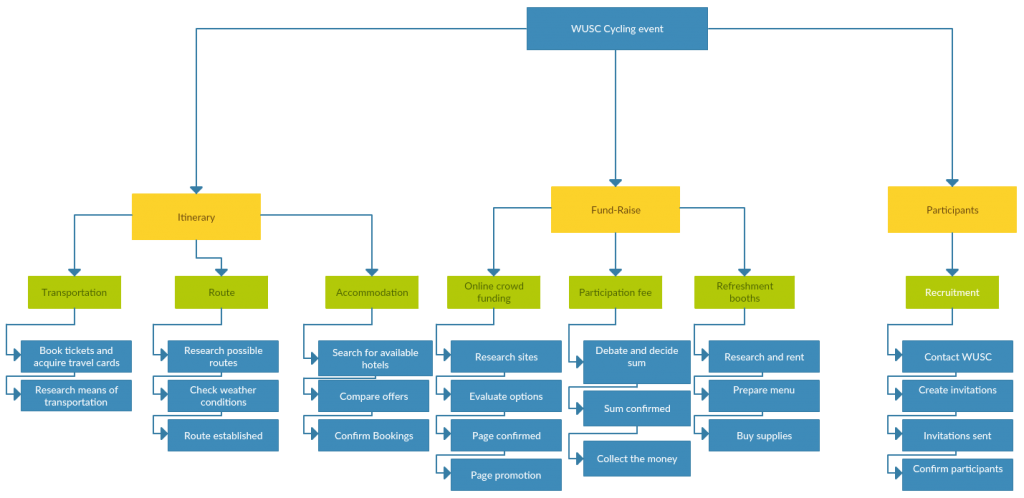
\includegraphics[width=\linewidth]{wbs-example-diag}
\end{figure}

\begin{figure}[!htb]
	\caption{Work Breakdown Structure Example (Hierarchy)}
	\label{fig:wbs-example-hier}
	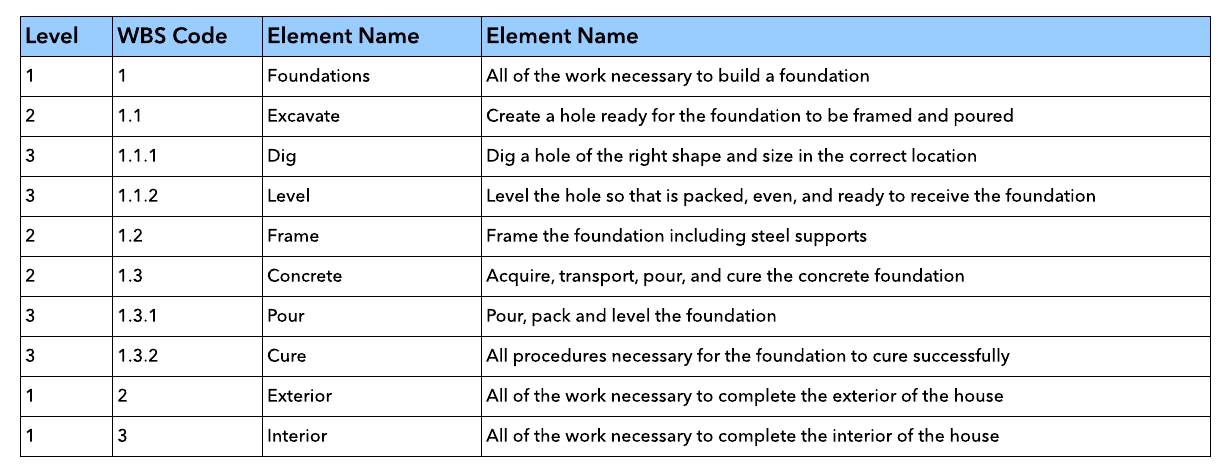
\includegraphics[width=\linewidth]{wbs-example-hier}
\end{figure}

	&& \textbf{Work package:} Unit of work which can be estimated, is a package which can be outsourced or contracted out, and produces a measurable deliverable
		&&& Smallest unit of a WBS
		&&& 8/80 hour rule: No work package should be less than 8 hours or more than 80 hours
		&&& Single reporting period rule: No set of work should be less than the reporting period (e.g. 2 weeks)
		&&& Should be sufficiently detailed to allow for cost and schedule estimates

\end{easylist}
\subsection{Network Diagram}
	\label{subsec:network-diagram}
\begin{easylist}

& \textbf{Network diagram:} Visual flow of the order in which work package are dependent on each other
	&& Conveys dependencies and chronological work order
	&& Conveys constraints such as:
		&&& Technical/causal constraint: Relationship between tasks where one task relies on the technical completion of the other
		&&& Management/discretionary constraint: Relationship between tasks where one task provides approval for the other to begin
		&&& Inter-project/resource constraint: Relationship between two tasks which are from separate areas (should be decoupled when possible to reduce risk)
		&&& Date constraint

\end{easylist}
\subsection{Estimations}
	\label{subsec:estimations}
\begin{easylist}

& \textbf{Top-down estimate:} Resource requirement estimate created from the requirements of top management
	&& Involves finish date, budget, resources, etc.
& \textbf{Bottom-up estimate:} Resource requirement estimate created from the analyses of the project manager and workers
& \textbf{Analogous estimate:} Resource requirement estimate created using a previous similar project
	&& \textbf{Parametric estimate:} Resource requirement estimate created using historical data with a multiplier for inflation, price increases, and other costs

& \textbf{Three Point Estimation:} Estimate generated from the weighted average of the most likely, pessimistic, and optimistic estimates

\end{easylist}
\begin{align*}
	TPE &= \frac{L + P + O}{3} \\
	\textrm{where } L &= \textrm{ most likely estimate} \\
	P &= \textrm{ pessimistic estimate} \\
	O &= \textrm{ optimistic estimate}
\end{align*}
\begin{easylist}

& Accuracy of estimates:
	&& \textbf{Ballpark estimate:} Estimate created with little time or information, and little accuracy (within 30\%)
	&& \textbf{Definitive estimate:} Estimate created with defined scope (within 5\%)

\end{easylist}
\clearpage

















	%
% BUS 361: Project Management - A Course Overview
% Section: Cost and Resource Management
%
% Author: Jeffrey Leung
%

\section{Cost and Resource Management}
	\label{sec:cost-resource-management}
\begin{easylist}

& \textbf{Effort:} Actual time invested in an activity (e.g. man hours)
& \textbf{Duration:} Time between activity start and finish

& Process to calculate resource cost:
	&& Create a WBS document
	&& Effort:
		&&& Create an estimate for total effort of all work packages
		&&& Multiply effort by resource cost
	&& Cost:
		&&& Create an estimate for total cost of all work packages
		&&& Apply contingency to effort and cost

& Types of costs:
	&& \textbf{Direct:} Costs which are clearly assigned to the output
		&&& E.g. Labor, materials, subcontractors, equipment, facilities, travel
	&& \textbf{Indirect:} Costs from internal spending which indirectly translate to output
		&&& E.g. Overhead costs (utilities, taxes, insurance, maintenance, depreciation) or administration (advertising, salaries, sales, commissions)
	&& \textbf{Fully loaded rate:} Labor costs which are calculated using an overhead multiplier
	&& \textbf{Nonrecurring:} Charges which are applied once (e.g. preliminary analyses, training)
	&& \textbf{Recurring:} Charges which continue over the timeline (e.g. labor, material)
	&& \textbf{Fixed:} Charges which do not change with usage (e.g. leasing capital hardware)
	&& \textbf{Variable:} Charges which increase with usage (e.g. equipment degradation)
	&& \textbf{Normal:} Charges which are expected and agreed upon
	&& \textbf{Expedited:} Charges which are unplanned and occur to speed up completion

& \textbf{Gantt chart:} Diagram of project schedule with start and finish dates of summary elements
	&& Simple to create and read
	&& Can be used for control
	&& Does not display details, sequencing, path to completion
	&& Does not provide information on efficient resources usage

\end{easylist}
\subsection{Critical Path Method}
	\label{subsec:critical-path-method}
\begin{easylist}

& \textbf{Float/slack:} Amount of time an activity can be delayed without affecting the project
	&& \textbf{Free float:} Amount of time an activity can be delayed without affecting the following activity
	&& \textbf{Total float:} Amount of time an activity can be delayed without affecting project completion date

& \textbf{Critical path:} Sequence of activities which determines the shortest total duration of the project
	&& Given possible sequences of precedence activities, the longest path has no float and is the critical path

& Critical path method:
	&& Conduct a forward pass to determine earliest start/end activity times
	&& Conduct a backward pass to determine latest start/end activity times
	&& Calculate the possible slack for each item

& To shorten the critical path:
	&& Eliminate tasks
	&& \textbf{Crashing:} Speeding up a task to reduce project duration
		&&& Shorten all/early/long/easy tasks, or tasks which cost less to speed up
	&& Overlap sequential tasks
		&&& \textbf{Fast tracking:} Allow parallel work

& Process to create a schedule:
	&& Using the effort calculated, create duration estimates
	&& Create a network diagram
	&& Generate a critical path from the network diagram
	&& Take the total duration from the critical path

\end{easylist}
\clearpage

	%
% BUS 361: Project Management - A Course Overview
% Section: Communications Management
%
% Author: Jeffrey Leung
%

\section{Communications Management}
	\label{sec:communications-management}
\begin{easylist}

& \textbf{Project plan:} Living document which describes the execution, monitoring, and control methods of the project
	&& Directs and allows management of objectives
	&& Built in collaboration with the team

& \textbf{Project communication:} Strategic management process for which the project manager is responsible
	&& Can alter behaviour
	&& Source of the communication is encoded into a message, conveyed in a medium, and decoded by the receiver
		&&& Can be altered by competing messages, noise, confusion, or other factors in between
	&& Difficult to quantify in results

& \textbf{Communications plan:} Schedule of how and when to communicate with stakeholders
	&& Methods of organization:
		&&& Events and times (e.g. milestones)
		&&& Documentation (e.g. charter, reports, closing document)
		&&& Stakeholders (see subsection~\ref{subsec:stakeholders})
			&&&& Stakeholders section may include owner

& Defining the information exchange with a stakeholder:
	&& Audience/target: Who is the stakeholder?
	&& Document format/content: What information is needed?
	&& Frequency/timing: When/how often will they need the information?
	&& Channel: How will the information be conveyed?
	&& Owner/contact: Who conveys the information?

\end{easylist}
\subsection{Stakeholders}
	\label{subsec:stakeholders}
\begin{easylist}

& \textbf{Stakeholder creep:} Phenomenon of people/organizations adding themselves to the group of stakeholders in order to be relevant

& Include those who:
	&& Control the scope
	&& Provide permission
	&& Complete the work
	&& Provide resources (e.g. supplies, people, time)
	&& Benefit or detract from the results

& \textbf{RACI analysis:} Accountability plan which maps tasks to the roles of stakeholders
	&& Conveys roles and responsibilities across organizational boundaries
	&& \textbf{R - Responsible:} Person responsible for performing a task
		&&& Ideally one person
	&& \textbf{A - Accountable:} Person accountable for the results of a task
		&&& Ideally one person
		&&& Can be same person as R
	&& \textbf{C - Consulted:} Person who must know and/or provide information before the task begins
		&&& Minimize to limit dependencies and speed up processes
	&& \textbf{I - Informed:} Person who must be notified after the task ends
	&& Process:
		&&& Identify stakeholders
		&&& Define tasks
		&&& Create a matrix with stakeholders and tasks
		&&& Assign RACI roles
		&&& Analyze the matrix horizontally (through tasks) to ensure:
			&&&& At least one person is Responsible
			&&&& At least one person is Accountable
			&&&& There are not too many people who must be Consulted
			&&&& There are not too many people who must be Informed
		&&& Analyze the matrix vertically (through stakeholders) to ensure:
			&&&& No one person has too many tasks for which they are Responsible
			&&&& No one person has too many tasks for which they are Accountable

\end{easylist}
\clearpage

	%
% BUS 361: Project Management - A Course Overview
% Section: Risk Management
%
% Author: Jeffrey Leung
%

\section{Risk Management}
	\label{sec:risk-management}
\begin{easylist}

& \textbf{Risk:} Uncertain event or condition which affects a project objective positively or negatively
	&& Often occurs when assumptions are made
	&& Types of risk: Financial, technical, commercial success, execution, contractual/legal

& \textbf{Risk management:} Identification, analysis, response to, and monitoring of risk factors
	&& Maximization of positive events, and minimizing likelihood and consequences of negative events

& Methods of identifying risk:
	&& WBS analysis
	&& Reviews of scope, stakeholders, and documents
	&& SWOT analysis
	&& Interviews and research

& Process of assessing risk:
	&& Identify probability of occurrence and potential consequences (both on a scale of Low, Guarded, Moderate, High, or Extreme)
	&& Equation: Event risk = Probability $\times$ Consequences
	&& Subjective
	&& \textbf{Probability/Likelihood Impact Matrix:} Organizational tool to graph the likelihood and consequences of risks for prioritization and comparison

& Responses to risk:
	&& \textbf{Avoidance:} Eliminating or limiting a risk through modifying limitations
	&& \textbf{Mitigation:} Eliminating or limiting a risk through limiting the probability or impact of a risk (e.g. simplifying processes, adding tests)
	&& \textbf{Transfer:} Eliminating or limiting a risk through shifting ownership or responsibility of the risk to another entity (e.g. warranties, contracts with fixed cost pricing)
	&& \textbf{Acceptance:} Eliminating or limiting a risk through being ready for the consequences (e.g. contingencies, fall-back plans, and workarounds)
	&& May alter WBS, network diagram, budget, scope, contingency reserves, etc.

& Monitoring risk:
	&& \textbf{Risk register:} Document which tracks risks, analyses, and response plans
	&& Monitor and report regularly (at least once per month)
	&& Stay updated on timelines for monitoring risks
	&& Track higher risks more frequently/closely

\end{easylist}
\clearpage

	%
% BUS 361: Project Management - A Course Overview
% Section: Quality Management
%
% Author: Jeffrey Leung
%

\section{Quality Management}
	\label{sec:quality-management}
\subsection{Quality Standards and Control}
	\label{subsec:quality-standards-control}
\begin{easylist}

& \textbf{Project quality:} Degree to which characteristics fulfill requirements
	&& \textbf{Grade:} Classification of a product based on its technical characteristics
	&& Low-grade may be acceptable; low-quality is unacceptable

& \textbf{Quality management process (PMBOK):} Ensuring that requirements are validated and met by customer
	&& Steps:
		&&& Identification of relevant quality standards and how to satisfy them through:
			&&&& Quality objectives (in Scope Document)
			&&&& Stakeholder expectations
			&&&& Product descriptions
			&&&& Standards/regulations
			&&&& Internal policies/objectives
		&&& Application and assurance of quality standards
		&&& Control and analyzing of quality using tools and techniques such as:
			&&&& Audits
			&&&& Adherence to guidelines
			&&&& Statistical sampling
			&&&& Inspection
			&&&& Graphs (e.g. flowcharts, histograms, scatterplots, pareto charts, fishbone diagrams)

& Trade-offs between scope, quality, cost, and schedule to avoid:
	&& Overwork resulting in mistakes and delays
	&& Rushing quality inspections resulting in undetected errors
	&& Exceeding quality objectives resulting in unbudgeted higher costs
	
& ISO Quality Management Framework:
	&& Customer satisfaction: Extent to which customers' needs and expectations are fulfilled
		&&& Involves requirement fulfillment and functional/emotional benefits of use
	&& Prevention over inspection: Concept of increasing cost over time to fix a lack of quality
	&& Responsibility of management to support
	&& Continuous improvement (Plan-Do-Check-Act cycle)

\end{easylist}
\subsection{Team Management}
	\label{subsec:team-management}
\begin{easylist}

& Structure project around meetings and events

& Holding meetings:
	&& Decide who should attend
	&& Set an agenda
	&& Communicate progress, problems, frustrations, and solutions
	&& Assign action items
	&& Be brief

& Purposes of status reporting:
	&& Raising issues
	&& Resolving problems
	&& Visibility of progress and work
	&& Accountability of work

& Role of the project manager:
	&& Manage human resources
	&& Manage connections with third parties
	&& Enforce task completion and ownership

\end{easylist}
\clearpage

	%
% BUS 361: Project Management - A Course Overview
% Section: Human Resources
%
% Author: Jeffrey Leung
%

\section{Human Resources}
	\label{sec:human-resources}
\begin{easylist}

& Planning resourcing:
	&& Create positions with skills, requirements
	&& Chart hierarchy
	&& Procure and assign resources

& \textbf{Project team:} Group of two or more people who share goals, are interdependent, have complementary skills, and are mutually accountable

& Characteristics of effective teams:
	&& Commitment to a goal or purpose
	&& Morale, team spirit
	&& Synergistic work
	&& Complementary skills
	&& Support

& \textbf{Tuckman's Team Development Stages:}
	&& \textbf{Formation:} Stage of team development when the team gets to know each other with awkwardness and miscommunication
		&& Agreed-upon points: Structure, goals, direction, roles
	&& \textbf{Storming:} Stage of team development when the team disagrees and resolves conflicts about the abilities to meet the goal
	&& \textbf{Norming:} Stage of team development when the team communicates well, resolves problems, becomes comfortable, and accepts teamwork
	&& \textbf{Performing:} Stage of team development when the team works independently and adaptively, can solve problems well, and has high morale
	&& \textbf{Adjourning:} Stage of team development when the team is recognized for achievements, says personal goodbyes

& Team development techniques:
	&& Team building activities
	&& Training
	&& Delegation
	&& Reward and recognition systems

\end{easylist}
\subsection{Motivation}
	\label{subsec:motivation}
\begin{easylist}

& \textbf{Motivation:} Intensity, direction, and persistence towards a goal

& \textbf{Extrinsic motivation:} Motivation based on earning a reward or avoiding a punishment
& \textbf{Intrinsic motivation:} Motivation based on a personal and internal reward

& \textbf{Maslow's Hierarchy of Needs:} Priorization of needs which must be fulfilled in the order of physiological, security, social, esteem, and self-actualization
& \textbf{McLelland's Three-Needs Theories:} Motivations are derived from aspirations toward achievement, power, or affiliation, one of which is primary
& \textbf{Theory X, Y:} $X$: People dislike work and responsibility and must be coerced, $Y$: People enjoy work, are creative, and want autonomy and responsibility
& \textbf{Expectancy Theory:} Motivation of effort results in increased performance which leads to higher value rewards/results
& \textbf{Adams' Equity Theory:} Motivation comes from perceived fairness, and inequities in input or output ratios will affect motivation
	&& Social comparison processes skews perceptions of equity

& Conflict:
	&& \textbf{Task conflict:} Conflict over project goals
	&& \textbf{Process conflict:} Conflict over the process of how work is carried out
	&& \textbf{Relationship conflict:} Conflict over interpersonal relationships
	&& \textbf{Functional conflict:} Conflict which improves the team (e.g. low level of task/process conflict)
	&& \textbf{Dysfunctional conflict:} Conflict which is harmful to the team (e.g. relationship conflict, high level of task/process conflict)

\end{easylist}
\clearpage

	%
% BUS 361: Project Management - A Course Overview
% Section: Controlling
%
% Author: Jeffrey Leung
%

\section{Controlling}
	\label{sec:controlling}
\begin{easylist}
	
& \textbf{Scope control:} Permitting only changes which are agreed upon
	&& \textbf{Scope creep:} Uncontrolled changes to project scope
	&& Change Control Process used to process requested scope changes and corrective actions
& \textbf{Schedule control:} Process of controlling project schedule changes
	&& Determine current status, determine influencing factors of schedule changes, identify schedule changes, and manage changes
	&& Tools: Progress reports, performance measurement, software
& \textbf{Cost control:} Process of controlling project cost changes

& Methods of project control:
	&& \textbf{Project/activity log:} Document recording occurrences throughout the project
	&& Progress/status report: Consistent recurring communication to stakeholders on project status
	&& Measurements
		&&& \textbf{Earned Value:} Technique to analyze variance of project performance (technical/scope, schedule/time, and cost)
			&&&& Budgeted Cost at Completion (BAC): Total budget for the project
			&&&& \textbf{Planned Value (PV):} Total budgeted cost for an activity
			&&&& \textbf{Actual Cost (AC):} Cost spent so far for an activity
			&&&& \textbf{Earned Value (EV):} Value of the work performed so far for an activity, based on the total project budgeted cost
				&&&&& Equation: $EV = BAC \times \textrm{Percentage completed}$
			&&&& \textbf{Cost Variance (CV):} Difference between Earned Value and Actual Cost
				&&&&& Equation: $CV = EV - AC$
			&&&& \textbf{Schedule Variance (SV):} Difference between Earned Value and Planned Value
				&&&&& Equation: $SV = EV - PV$
			&&&& \textbf{Cost Performance Index (CPI):} Ratio of Earned Value to Actual Cost
				&&&&& Equation: $CPI = \frac{EV}{AC}$
			&&&& \textbf{Schedule Performance Index (SPI):} Ratio of Earned Value to Planned Value
				&&&&& Equation: $SPI = \frac{EV}{PV}$

\end{easylist}
\clearpage

	%
% BUS 361: Project Management - A Course Overview
% Section: Closeout
%
% Author: Jeffrey Leung
%

\section{Closeout}
	\label{sec:closeout}
\begin{easylist}

& Finish all deliverables
& Receive client sign-off/acceptance
& Conduct post-implementation audit
	&& Often received by senior management
	&& Contents:
		&&& Whether the goal was achieved
		&&& Whether the project was on time and on budget
		&&& Whether the client was satisfied
		&&& Whether the business value was realized
		&&& Lessons learnt - what should be done again, what should not be done
& Collect documentation
	&& Includes charter, scope, design documents, status reports, meeting minutes, change requests, client acceptance, audit report
	&& Used for:
		&&& Reference for future changes
		&&& Team performance evaluation
		&&& History of resource use (costs and duration)
		&&& History of issues
		&&& Training for other workers
		&&& Templates for future work
& Create final project report
	&& Overall success and criteria
	&& Organization and affiliations of project
	&& Strengths and weaknesses
	&& Recommendations from team

\end{easylist}
\clearpage

	%
% CMPT 310: Artificial Intelligence - A Course Overview
% Section: Flashcard Questions
%
% Author: Jeffrey Leung
%

\section{Flashcard Questions}
	\label{sec:flashcard-questions}
\begin{easylist}

& What characteristics does a task environment consist of?
	&& Performance measure, Environment, Actuators, Sensors (PEAS)
& What does a problem formulation consist of?
	&& Initial state, goal test, successor function, and cost function

& How is uniform-cost search different from breadth-first search?
	&& Uniform-cost search uses a priority queue to follow the path of least cost
& Which search algorithm is iterative deepening search derived from?
	&& Depth-first search
& How is iterative deepening search unique?
	&& Maximum depth of depth-first search increases until the goal is found

& What is an admissible heuristic?
	&& Function which underestimates the true cost to the goal
& What is a dominant heuristic?
	&& Admissible heuristic which is greater than or equal to another admissible heuristic
& How is greedy/heuristic search different from A* search?
	&& Heuristic search does not consider the distance already travelled
& What is the equation for A* search?
	\end{easylist}
	\begin{align*}
		f(n) & = g(n) + h(n) \\
		\textrm{where }
		& f(n) = \textrm{ estimated total cost of the path through } n \textrm{ to the goal} \\
		& g(n) = \textrm{ cost so far to reach } n \\
		& h(n) = \textrm{ heuristic-estimated cost from } n \textrm{ to the goal}
	\end{align*}
	\begin{easylist}

& Which of $\alpha / \beta$ is the upper bound on the potential minimum node, and which is the lower bound on the potential maximum node?
	&& $\alpha$: Lower bound on the potential value of a maximum node
	&& $\beta$: Upper bound on the potential value of a minimum node

& When does backtracking search backtrack?
	&& When a variable has no possible valid values, given the assignments of the other variables
& What algorithm is DPLL derived from?
	&& Backtracking search
& How does WalkSAT `walk'?
	&& The value of a random variable from a false clause is flipped

& What is a normalization constant?
	&& A value which every probability is divided by, to reduce a probability function to a total probability of 1
& What is the difference between dependence and conditional dependence?
	&& Dependence: Whether knowing a variable has an effect on the probability of another variable (share a parent node in Bayesian network)
	&& Conditional dependence: Given an evidence variable(s), whether knowing a variable has an effect on the probability of another variable (share a child node in Bayesian network)
& What is the formula for the Chain Rule?
	\end{easylist}
		\begin{align*}
		P(a, b) &= P(a) P(b|a) = P(b) P(a|b) \\
		P(x_1, \dotsc, x_n) &= \prod_{i=1}^n P(x_i | x_1, \dotsc, x_{i-1})
		\end{align*}
	\begin{easylist}

& What is the formula for Bayes' Rule?
	\[
		P(B | A) = \frac{P(A | B) \times P(B)}{P(A)}
	\]
	
& What is rejection sampling?
	&& Sampling each variable multiple times to find approximate probabilities of all variables
& What is Gibbs sampling?
	&& Fixing evidence variables, randomly assigning values to non-evidence variables, sampling a non-evidence variable, and iterating through all non-evidence variables

& What is filtering?
	&& Finding a hidden probability given evidence of all previous probabilities (i.e. finding $x_t$ given $e_{1:t}$)
& What is smoothing?
	&& Finding previous hidden probabilities given evidence of previous and future probabilities (i.e. finding $x_t$ given $e_{1:T}$ where $1 <= t < T$)
& What does the Viterbi algorithm do?
	&& Find the most likely sequence of states ending in xt

& How do you avoid overfitting?
	&& Use relatively less training data

& What is the equation used for entropy?
	&& $H(p_1, p_2, \dotsc, p_n) = - \sum_i p_i \log_2 p_i$
& What is the equation used for reduction in uncertainty?
	&& $H(root) - \sum_{i \in \textrm{children}} \frac{\textrm{samples of } i}{\textrm{samples of root}} H(i)$
& What is the entropy of a 50/50 choice?
	&& 1
& What is the entropy of a 0/100 choice?
	&& 0
& Do you make a choice at a decision tree to increase or decrease entropy?
	&& Decrease entropy (i.e. maximize reduction of entropy)

& What is the equation for a threshold function?
	\end{easylist}
	\[
		a = \begin{dcases}
			-1 & \textrm{if } in < 0 \\
			1 & \textrm{otherwise}
		\end{dcases}
	\]
	\begin{easylist}

& What is the equation for a ReLU function?
	\end{easylist}
	\[
		a = max(0, in)
	\]
	\begin{easylist}

\end{easylist}
\clearpage


\end{document}
